\section{BAO fits}
\label{sec:fits}

\textcolor{red}{one or two options for the model. nuisance parameters.}

\textcolor{red}{Glam template. Linear template.}

\textcolor{red}{spread of measured alpha over 25 FirstGens}

\textcolor{red}{alongside with alpha fits to the power spectrum}

\textcolor{red}{experiment with some choices.}

\textcolor{red}{sigma alpha from the posterior (as a function of k)}

\textcolor{red}{min $\chi^{2}$ vs alpha for P(k), B(k1, k2, k3), P+B BAO and BAOless templates. Look into the scatter in the detection significance across the realizations.}

% \begin{figure*}
% 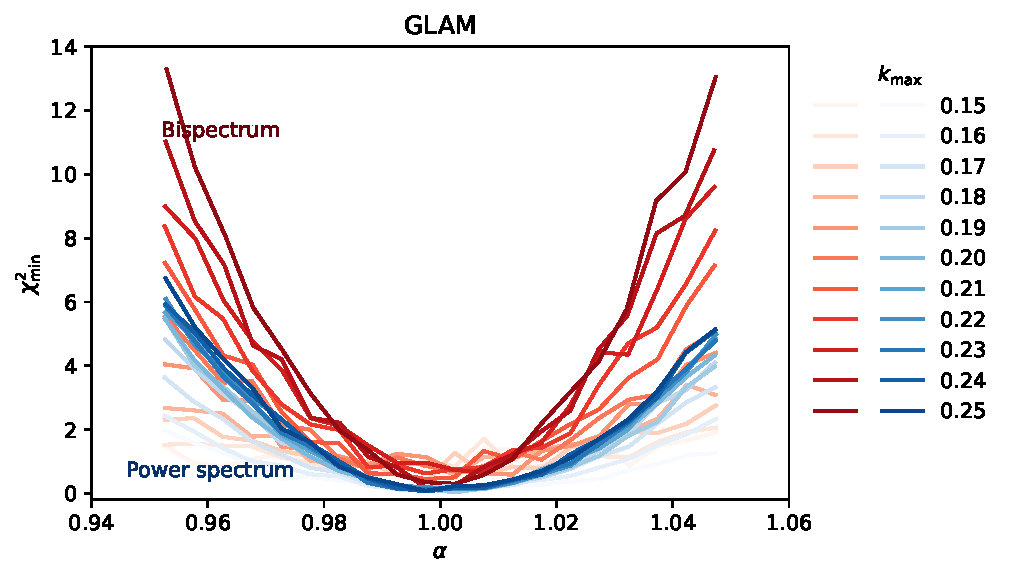
\includegraphics[width=0.48\textwidth]{chi2_GLAM.pdf}
% 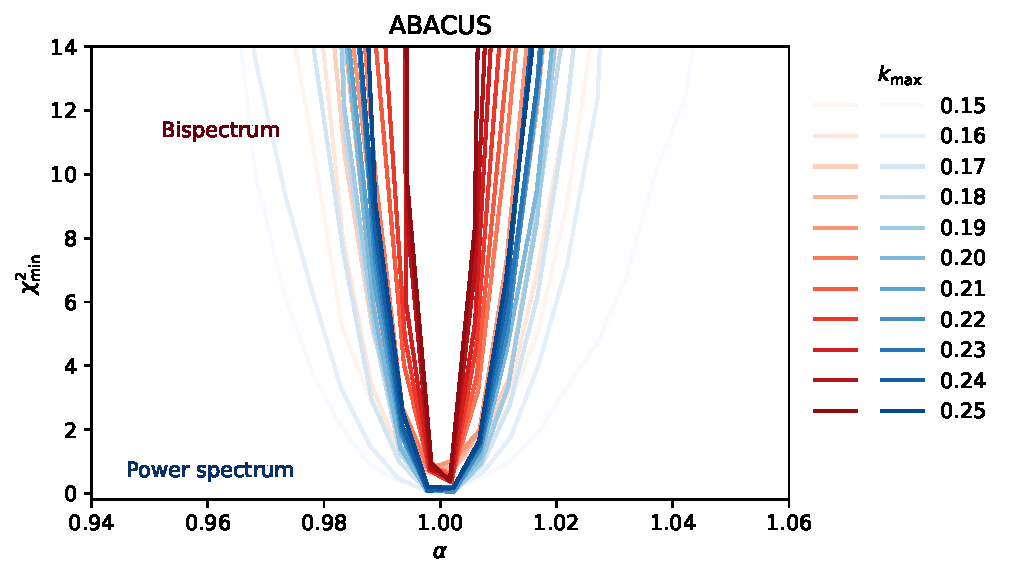
\includegraphics[width=0.48\textwidth]{chi2_ABACUS.pdf}
% 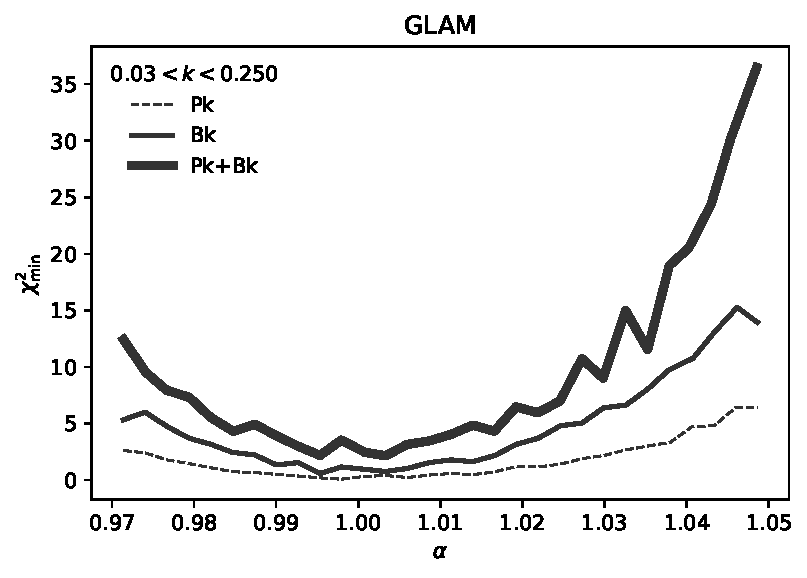
\includegraphics[width=0.48\textwidth]{chi2alpha_glam.pdf}
% 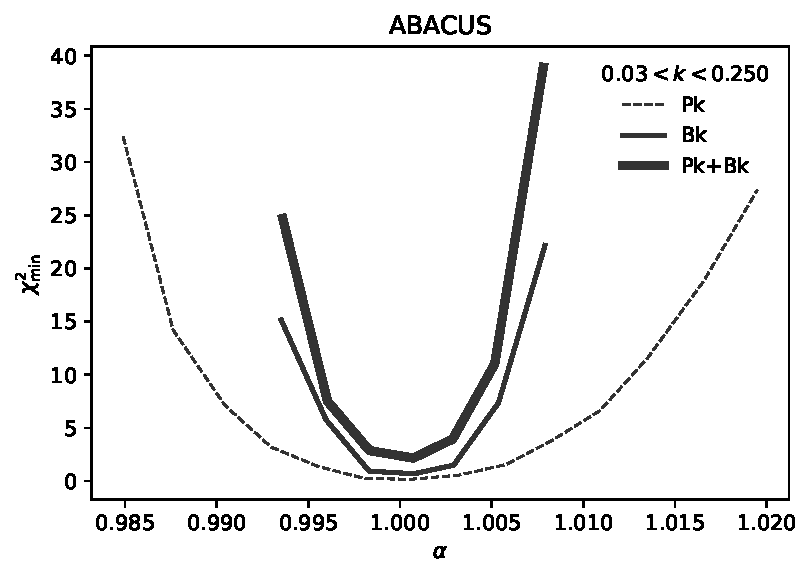
\includegraphics[width=0.48\textwidth]{chi2alpha_abacus.pdf}
% \caption{Marginalized minimum $\chi^{2}$ as a function of the BAO peak $\alpha$}\label{fig:chi2alpha}
% \end{figure*}

% \begin{figure*}
% 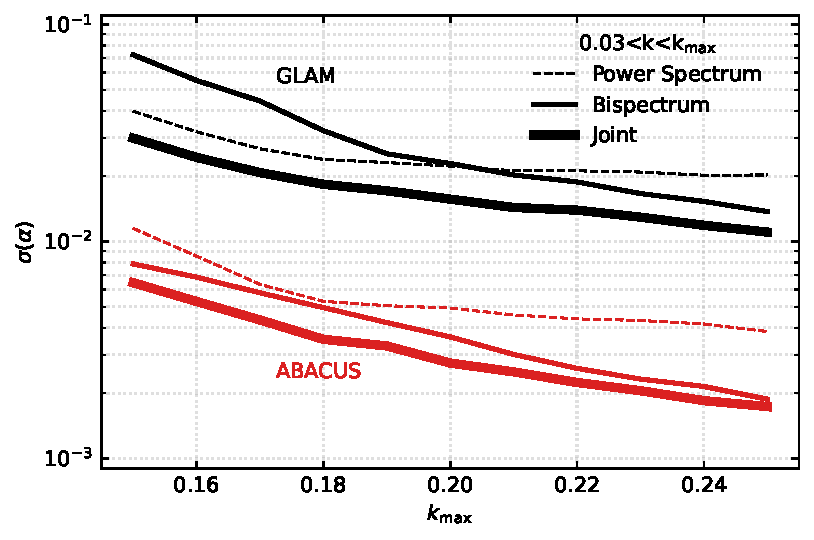
\includegraphics[width=0.9\textwidth]{sigma_kmax.pdf}
% \caption{Dispersion in the BAO peak $\alpha$ as a function of the maximum wavenumber $k_{\rm max}$}
% \end{figure*}